
\textbf{\underline{В первой главе}} представлены обзор и анализ областей, которые необходимы для решения поставленных научных задач.

Была проведена классификация машин, использующих ноги в качестве движителя. По результатам классификации объектом исследования является многоногая шагающая машина с движителями циклического действия. Изучив данный класс машин были осмыслены габаритные и структурные особенности этих роботов.

Так как основным местом применения разработанных методов предполагается исследование пещер роботами, то были рассмотрены типы роботов и робототехнических систем, которые могут использоваться для изучения поверхности пещер.

Для решения задачи определения геометрических и физико-механических свойств пройденной поверхности необходимо понимать в каких условиях будет использоваться робот: типы препятствий и размеры. В пещерах встречаются следующие типы поверхностей: твердые породы, прочные (мрамор), мягкие (мел, известняк); сыпучие грунты (песок); водные преграды (лужи, бассейны); скользкие и упругие поверхности (мох, плесень); пластинчатые (земля). С точки зрения механики все эти типы поверхностей могут характеризоваться их свойствами упругости, в/вязкости и пластичности. Длины многих пещер измеряются километрами, а их габариты очень сильно варьируются от нескольких сантиметров, до многих километров в ширину. Однако наибольший интерес в контексте исследования представляют проходы шириной в несколько десятков сантиметров, потенциально доступные, но опасные для человека.

Задача определения геометрических свойств объекта является частью Mapping из  класса методов Simultaneous Localization and Mapping (SLAM). По результатам анализа известных методов сделан высвод, что задача локализации может быть решена с помощью маяков или ToF камеры, но для построения карты требуется разработка собственного метода.

Проведен обзор алгоритмов триангуляции, так как данный метод лёг в основу определения геометрических свойств объекта. Была выявлена необходимость разработки модифицированного метода 2D триангуляции Делоне для вогнутых оболочек.

Были рассмотрены различные алгоритмы и средства определения физико-механических свойств поверхности. Сделан вывод о необходимости использования датчика силы, установленного на ногу робота, а также собирать дополнительные данные об угловой скорости и моменте на моторе.

Для решения задачи оптимизации количества ног робота, выявлена необходимость генерировать семейства поверхностей с одинаковой сложностью. Поиск различных вариантов привел к выбору подхода <<Получение искусственных поверхностей на основе параметров генерации>>, который был модифицирован автором.

На основе литературного обзора было выявлено, что предложенные решения для определения геометрических и физико-механических свойств не встречается в научных публикациях российских и зарубежных авторов, следовательно обладают признаками новизны.

На основе проведенного анализа, разработана концепция робота \pic{fig:diag_system.png}. Оранжевым цветом выделены компоненты системы, которые представляют собой предмет исследования в рамках диссертационной работы. Голубым цветом выделены блоки которые были использованы в работе как стандартные средства, без каких-либо существенных доработок.
\begin{figure}[ht!]
    \centering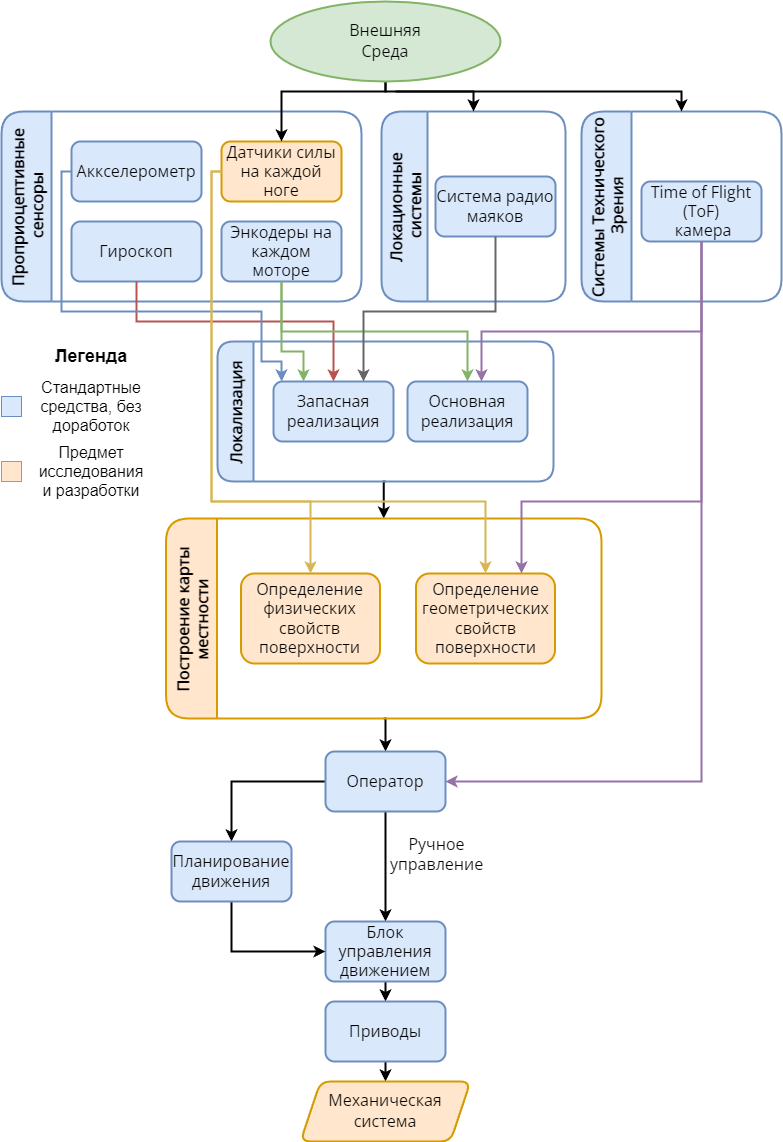
\includegraphics[height=15cm,width=1\textwidth,keepaspectratio]{main_diag.drawio.png}
    \caption{Структурная схема разработанной системы}
    \label{fig:diag_system.png}
\end{figure}


